
%----------------------------------------------------------------------------------------
%	PACKAGES AND DOCUMENT CONFIGURATIONS BY DANIEL HEDIGER
%----------------------------------------------------------------------------------------

\documentclass{article}

\usepackage[version=3]{mhchem} % Package for chemical equation typesetting
\usepackage{siunitx} % Provides the \SI{}{} and \si{} command for typesetting SI units
\usepackage{graphicx} % Required for the inclusion of images
\usepackage{natbib} % Required to change bibliography style to APA
\usepackage{amsmath} % Required for some math elements 
\usepackage{german}
\usepackage{float}
\restylefloat{figure}
\usepackage[utf8]{inputenc}
\setlength\parindent{0pt} % Removes all indentation from paragraphs
\renewcommand{\labelenumi}{\alph{enumi}.} % Make numbering in the enumerate environment by letter rather than number (e.g. section 6)
\usepackage{blindtext}

%\usepackage{times} % Uncomment to use the Times New Roman font

%----------------------------------------------------------------------------------------
%	DOCUMENT INFORMATION
%----------------------------------------------------------------------------------------

\title{Physiklabor \\ Laborbericht \\ Optik} % Title

\author{Daniel \textsc{Hediger} \\ Lucien \textsc{Egloff}} % Author name



\date{\today} % Date for the report

\begin{document}

\maketitle % Insert the title, author and date

\begin{center}
\begin{tabular}{l r}
	Ausführungsdatum: & Dezember 7, 2016 \\ % Date the experiment was performed
	Dozent: & Dr.Ackermann \\% Instructor/supervisor
	Version: & 1.0
	
\end{tabular}
\end{center}
\begin{figure}[H]
	\centering
	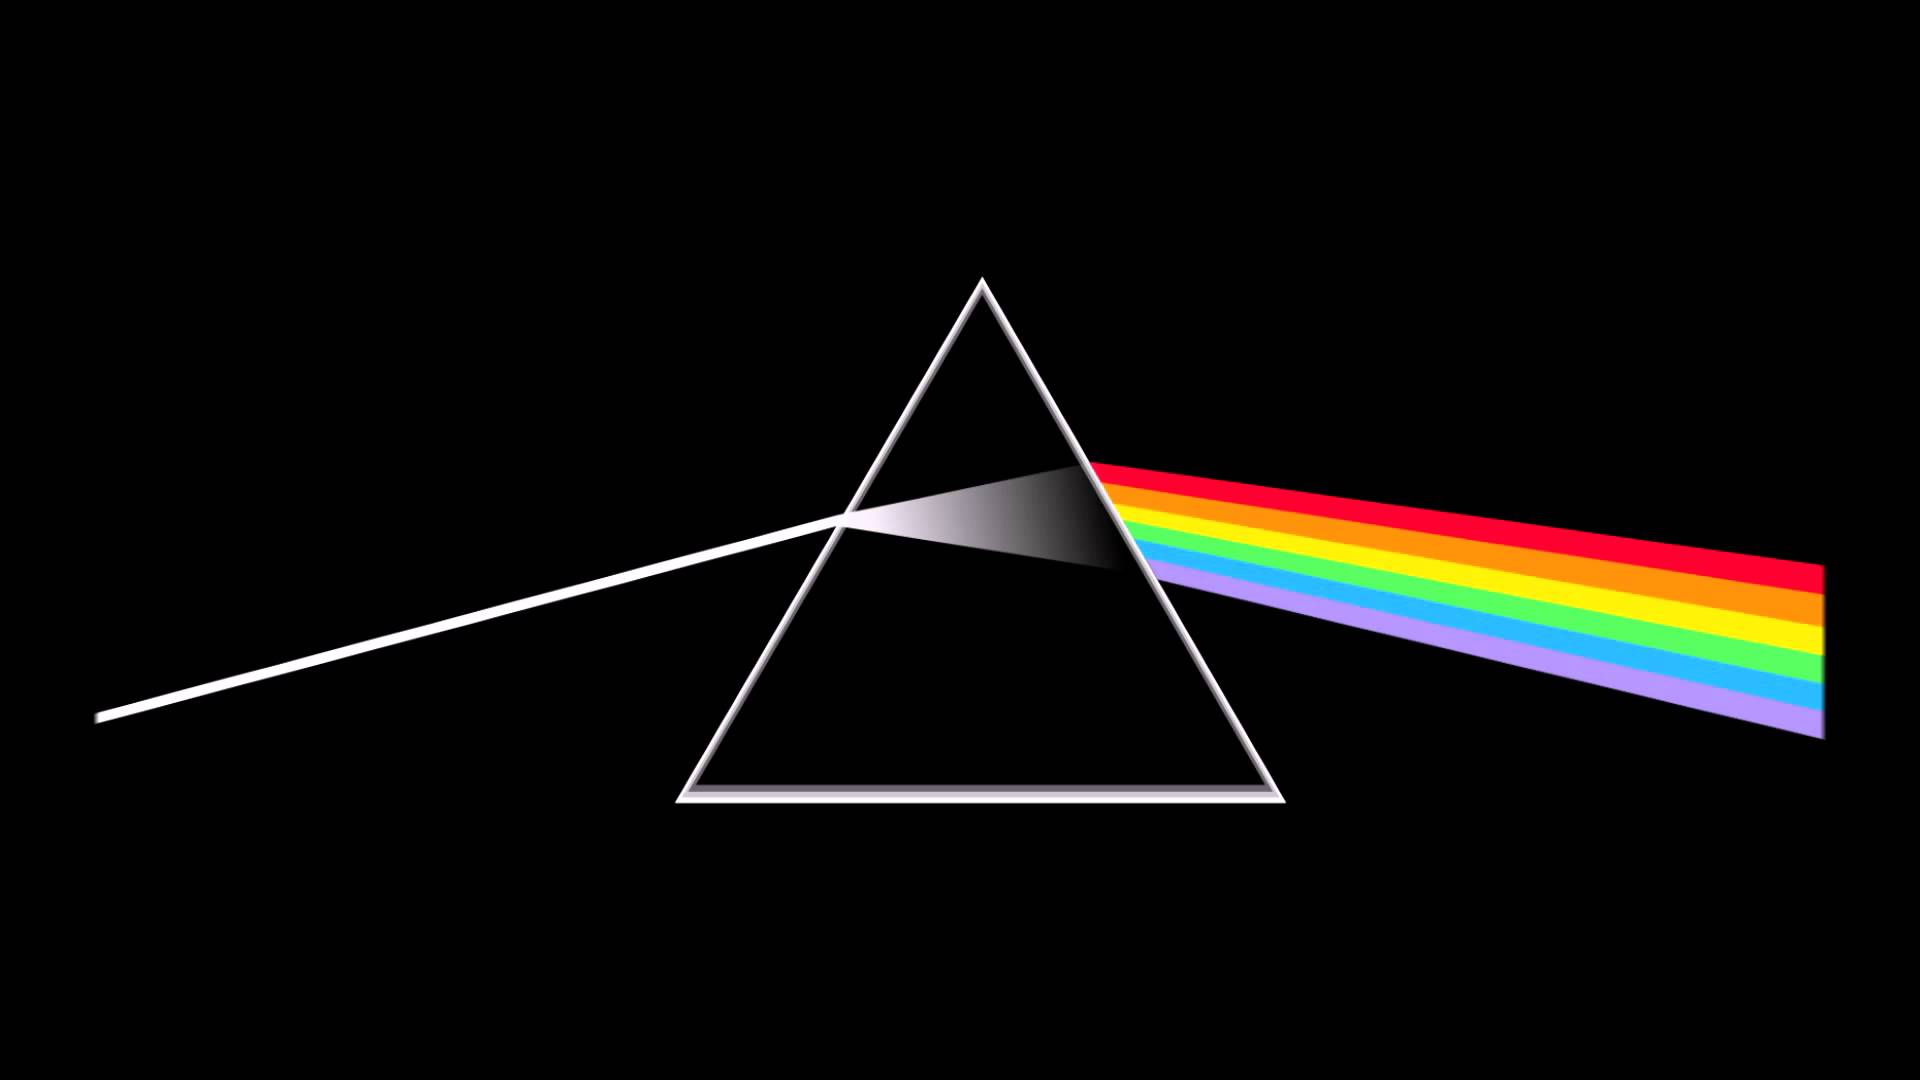
\includegraphics[scale=0.2]{dsotm.jpg} 
\end{figure}
\newpage
\tableofcontents 

%----------------------------------------------------------------------------------------
%	SECTION 1
%----------------------------------------------------------------------------------------
\newpage
\section{Versuch 1 Haardurchmesser}
\subsection{Versuch}
Es wurde mit einem grünen Laserstrahls auf ein Haar gehalten. Die Beugung der Lichtwellen konnte
man an der Wand im Hintergrund mit drei Maxima erkennen. Indem die Abstände der Maxima und
der Abstand der Wand gemessen wurde, konnte die Dickes des Haars berechnet werden. Der Versuch
wurde ebenfalls mit einer Kohlenfaser durchgeführt. Der Laserstrahl muss breiter sein als das
Objekt.
\subsection{Messwerte}

\textbf{Haar:}

\begin{tabular}{l r}
	Abstand des Maxima $\Delta$k & \textbf{45mm}\\
	k	&\textbf{1}\\
	Abstand zu Wand L&\textbf{3000mm} \\
	Wellenlänge Lasers $\lambda$ & \textbf{532nm}
\end{tabular}

\textbf{Kohlefaser:}

\begin{tabular}{l r}
	Abstand des Maxima $\Delta$k & \textbf{150mm}\\
	k	&\textbf{1}\\
	Abstand zu Wand L&\textbf{3000mm}\\
	Wellenlänge Lasers $\lambda$ & \textbf{532nm}
\end{tabular}

\subsection{Berechnungen}
\textbf{Haar}
\begin{equation}
\varphi = arctan(\frac{\Delta k}{L}) = \frac{45}{3000}
\end{equation}
\begin{equation}
L = \lambda \cdot \frac{k+0.5}{sin(\varphi)}= \underline{\underline{text}} 
\end{equation}
\textbf{Kohlefaser}
\begin{equation}
\varphi = arctan(\frac{\Delta k}{L}) = \frac{45}{3000}
\end{equation}
\begin{equation}
L = \lambda \cdot \frac{k+0.5}{sin(\varphi)}= \underline{\underline{text}} 
\end{equation}
\subsection{Fehlabschätzung}
\begin{tabular}{l r}
	Haardicke mit dem Mikrometer gemessen & \textbf{0.045mm}\\
	Kohlefaser mit dem Mikrometer gemessen	&\textbf{0.005mm}\\
\end{tabular}
\vspace{3mm}

Das Haar konnte ziemlich genau gemessen werden, bei der Kohlefaser kann es sein, dass ein Bündel
von Kohlefaser gemessen wurde, das es schwer war diese voneinander zu trennen.
\section{Versuch 2 Spurabstand CD/DVD}
\subsection{Versuch}
Der Spurabstand wurde durch die Reflektion des Laserstrahls und dessen Beugung ähnlich wie im
Haardurchmesser-Versuch ermittelt. Der grüne Laserstrahl trifft auf die Oberfläche der CD, dringt
durch die Gitterstruktur und Reflektiert an der Rückseite der CD. Die reflektierten Maxima konnten auf
eine Oberfläche in der Nähe des Lasergerätes projiziert werden. Es wurde wiederum der Winkel ermittelt,
und mit der Wellenlänge des Lasers der Spurabstand gerechnet. Weil es sich um eine Gitterstruktur
handelt muss beim Rechnen nicht 0.5 zum k addiert werden.
\subsection{Messwerte}
\begin{tabular}{l r}
	\textbf{CD:}&\\
Abstand des Maxima& \textbf{101mm}\\
L & \textbf{244mm}\\
	\textbf{DVD:}&\\
Abstand des Maxima& \textbf{435mm}\\
L & \textbf{400mm}
\end{tabular}
\subsection{Berechungen}
\textbf{CD:}
\begin{equation}
\varphi = arctan(\frac{\Delta k}{L}) =\underline{22.5^\circ}
\end{equation}
\begin{equation}
L = \lambda \cdot \frac{k+0.5}{sin(\varphi)}= \underline{1.4\mu m} 
\end{equation}
Anzahl Umgänge:
\begin{equation}
U = \frac{b}{L}=\frac{37}{1.4\mu m}= \underline{\underline{26`400}}
\end{equation}
\textbf{DVD:}
\begin{equation}
\varphi = arctan(\frac{\Delta k}{L}) =\underline{47.4^\circ}
\end{equation}
\begin{equation}
L = \lambda \cdot \frac{k+0.5}{sin(\varphi)}= \underline{0.72\mu m} 
\end{equation}
Anzahl Umgänge:
\begin{equation}
U = \frac{b}{L}=\frac{37}{0.72\mu m}= \underline{\underline{51`400}}
\end{equation}
\subsection{Fehlabschätzung}
Literaturwerte:\\

\begin{tabular}{l r}
\textbf{CD}& 1.6$\mu$ m\\
\textbf{DVD}	&0.7$\mu$ m\\
	
\end{tabular}
\vspace{3mm}\\
Die gemessenen Daten stimmen recht genau im Vergleich zum Literaturwert.
\newpage
\section{Versuch 3 Wellenlänge des roten Lasers}
\subsection{Versuch}
Mit dem gleichen Aufbau wie die CD und DVD gemessen wurde, wurde nun der Rote Laser eingespannt.
Jetzt wurde die Gleichung umgestellt und nach der Wellenlänge aufgelöst.
\subsection{Messwerte}
\begin{tabular}{l r}
	$\Delta$k & \textbf{482mm}\\
	L & \textbf{307mm}\\
	$\varphi$ & $57.5^\circ$
\end{tabular}
\subsection{Berechnungen}
\begin{equation}
\lambda = l \cdot sin(\varphi) = \underline{\underline{607nm}}
\end{equation}
\subsection{Fehlabschätzung}
Wellenlänge gemäss Aufdruck = \textbf{635nm}
 Die Abweichung ist relativ klein und beruhen von Messungenauigkeiten.
 \newpage
 \section{Aufgabe 4 Laserleistung}
 \subsection{Versuch}
 Der Laser wurde bei diesem Versuch auf eine Fotodiode gerichtet. An der Diode wurde über einen
 Widerstand von 500 Ohm die Spannung gemessen. Damit kann der Strom ermittelt werden. Mit der
 Tabelle der Diode konnte dann mit der Wellenlänge die Leistung pro Ampere abgelesen werden. Somit
 wurde die Leistung mit Strom und diesem Responsivity Wert aus der Tabelle ausgerechnet.
 \subsection{Messwerte}
 \begin{tabular}{l r}
 	\textbf{Laser Rot:}&\\
 	$\lambda$ & \textbf{635nm}\\
 	Spannung & \textbf{0.15V}\\
 	\textbf{Laser Grün:}&\\
 	$\lambda$ & \textbf{532nm}\\
 	Spannung & \textbf{0.116V}\\
 \end{tabular}
 \subsection{Berechnungen}
 \begin{figure}[H]
 	\centering
 	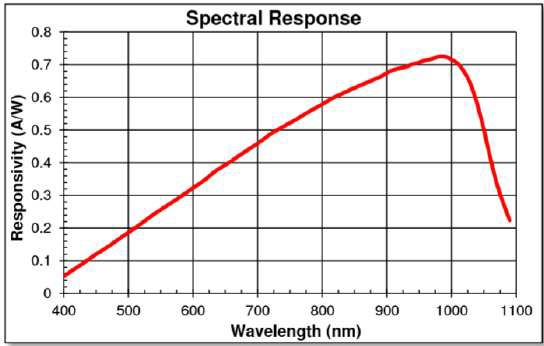
\includegraphics[width=0.9\textwidth]{SR}
 	\caption{Tabelle der Werte vom Photodetektor}
 \end{figure}
\newpage
\textbf{Roter Laser:}
\begin{equation}
I = \frac{U}{R}=\frac{0.15V}{500\Omega}= \underline{0.3mA} 
\end{equation}
\begin{equation}
Responsitive = = \underline{0.36A/m}
\end{equation}
\begin{equation}
P = \frac{I}{Responsitive}= \frac{0.3mA}{0.36A/m}= \underline{\underline{0.83mW}}
\end{equation}
\textbf{Roter Grün:}
\begin{equation}
I = \frac{U}{R}=\frac{0.116V}{500\Omega}= \underline{0.23mA} 
\end{equation}
\begin{equation}
Responsitive = = \underline{0.23A/m}
\end{equation}
\begin{equation}
P = \frac{I}{Responsitive}= \frac{0.23mA}{0.23A/m}= \underline{\underline{1mW}}
\end{equation}
\section{Versuch 5 Laser Polarisation}
\subsection{Versuch}
Jetzt wurde ein Polarisationsfilter zwischen Laser und Fotodiode eingebaut. Dieser Filter lässt nur die
senkrechten Wellen passieren wenn er senkrecht eingestellt ist. Der Filter lässt sich um $180^\circ$ verdrehen.
Alle Positionen des Filters wurden gemessen und danach aus dem Maximum und Minimum der
Leistung der Polarisationsgrad gerechnet.
\subsection{Messwerte}
\begin{tabular}{|c|c|c|}
	\hline 
	\textbf{Winkel}& \textbf{Spannung Rot$[mV]$} &\textbf{Spannung Grün$[mV]$}  \\ 
	\hline 
	-90& 41 & 64 \\ 
	\hline 
	-80& 25 &  59\\ 
	\hline 
	-70& 13 &  62\\ 
	\hline 
	-60&  5& 44 \\ 
	\hline 
	-50& 1 & 36 \\ 
	\hline 
	-40& 3 &  28.3\\ 
	\hline 
	-30&  10&22  \\ 
	\hline 
	-20& 22 & 19 \\ 
	\hline 
	-10& 36 & 20 \\ 
	\hline 
	0& 52 &23  \\ 
	\hline 
	10&  65& 29 \\ 
	\hline 
	20& 78 & 37 \\ 
	\hline 
	30& 88 & 45 \\ 
	\hline 
	40& 93 &  55\\ 
	\hline 
	50&  92&  62\\ 
	\hline 
	60& 86 & 68 \\ 
	\hline 
	70& 77 &  72\\ 
	\hline 
	80&  60& 72 \\ 
	\hline 
	90& 44 &  70\\ 
	\hline 
\end{tabular} 
\
\end{document}
\